\documentclass[10pt,twocolumn]{article}

% ── Geometry ──────────────────────────────────────────────────────────────────
\usepackage[top=0.6in,bottom=1in,left=0.6in,right=0.6in,columnsep=0.25in]{geometry}

% ── Fonts & Encoding ──────────────────────────────────────────────────────────
\usepackage[T1]{fontenc}
\usepackage[utf8]{inputenc}
\usepackage{lmodern}
\usepackage{microtype}

% ── Math ──────────────────────────────────────────────────────────────────────
\usepackage{amsmath,amssymb}

% ── Units ─────────────────────────────────────────────────────────────────────
\usepackage{siunitx}
\sisetup{
  per-mode          = symbol,
  detect-all,
  group-separator   = {,},
  group-minimum-digits = 4
}

% ── Tables ────────────────────────────────────────────────────────────────────
\usepackage{booktabs}
\usepackage{array}
\usepackage{tabularx}

% ── Figures ───────────────────────────────────────────────────────────────────
\usepackage{graphicx}
\usepackage{float}
\usepackage[labelfont=bf,font=small,format=plain]{caption}

% ── References & Links ────────────────────────────────────────────────────────
\usepackage{hyperref}
\hypersetup{
  colorlinks  = true,
  linkcolor   = black,
  citecolor   = black,
  urlcolor    = black,
  pdftitle    = {2D CPU/GPU Die Thermal Simulation},
  pdfauthor   = {Joey Kim}
}

% ── Section style ─────────────────────────────────────────────────────────────
\usepackage{titlesec}
\titleformat{\section}{\normalfont\bfseries\large}{\thesection.}{0.5em}{}
\titleformat{\subsection}{\normalfont\bfseries}{\thesubsection.}{0.5em}{}
\titlespacing*{\section}{0pt}{8pt}{4pt}
\titlespacing*{\subsection}{0pt}{6pt}{2pt}

% ── Header / Footer ───────────────────────────────────────────────────────────
\usepackage{fancyhdr}
\pagestyle{fancy}
\fancyhf{}
\renewcommand{\headrulewidth}{0.4pt}
\fancyhead[L]{\footnotesize\textit{2D CPU/GPU Die Thermal Simulation}}
\fancyhead[R]{\footnotesize\textit{Finite Difference Methods}}
\fancyfoot[C]{\footnotesize\thepage}

% ── Misc ──────────────────────────────────────────────────────────────────────
\usepackage{enumitem}
\setlist[itemize]{noitemsep,topsep=2pt}
\usepackage{parskip}
\setlength{\parskip}{2pt}

% ── Global spacing tightening ─────────────────────────────────────────────────
% Float separation (space between floats and text)
\setlength{\textfloatsep}{6pt plus 2pt minus 2pt}
\setlength{\floatsep}{4pt plus 2pt minus 2pt}
\setlength{\intextsep}{4pt plus 2pt minus 2pt}
% Caption spacing
\setlength{\abovecaptionskip}{3pt}
\setlength{\belowcaptionskip}{0pt}
% Equation spacing (global default)
\setlength{\abovedisplayskip}{3pt}
\setlength{\belowdisplayskip}{3pt}
\setlength{\abovedisplayshortskip}{1pt}
\setlength{\belowdisplayshortskip}{3pt}

% ==============================================================================
\begin{document}
% ==============================================================================

% ── Title block (one-column) ──────────────────────────────────────────────────
\twocolumn[{%
  \vspace{-12pt}%
  \begin{center}
    {\LARGE\bfseries%
      2D CPU/GPU Die Thermal Simulation\\[3pt]%
      Using Finite Difference Methods}\\[6pt]
    {\normalsize Jaehyeok Kim \quad\textbar\quad Georgia Institute of Technology}
  \end{center}
  \rule{\textwidth}{0.8pt}
  \vspace{4pt}
  \noindent\textbf{Abstract.}\quad\setlength{\parskip}{0pt}%
  This report presents a 2D transient and steady-state heat transfer
  simulation of a multi-layer CPU/GPU chip package using finite difference
  methods (FDM). Three numerical solvers are implemented in MATLAB: an
  explicit forward-time central-space (FTCS) scheme, an implicit
  backward-time central-space (BTCS) scheme solved with Gauss--Seidel
  iteration, and a direct steady-state Gauss--Seidel solver.
  The domain models three physical layers---silicon die, thermal interface
  material (TIM), and copper heat spreader---with three localized
  volumetric heat sources at $\dot{q}''' = \SI{5e8}{W/m^3}$ representing
  CPU cores. Convective cooling ($h = \SI{2000}{W/m^2.K}$) is applied at
  the top and lateral boundaries with an adiabatic bottom.
  Peak junction temperatures, layer-to-layer thermal gradients, and
  cool-down dynamics are characterized. All three solvers converge to the
  same steady-state distribution, validating the numerical implementation.
  \vspace{4pt}
  \rule{\textwidth}{0.4pt}
  \vspace{6pt}
}]

% ==============================================================================
\section{Introduction}
% ==============================================================================

Thermal management is a critical design constraint in modern
microelectronics. As transistor densities increase, localized heat fluxes
can exceed \SI{100}{W/cm^2}, elevating junction temperatures that degrade
device reliability and performance. Accurate thermal modeling enables
engineers to evaluate heat spreader geometry, thermal interface materials,
and cooling strategies before physical prototyping.

This simulation studies a cross-sectional slice of a representative
CPU/GPU chip package under worst-case operating conditions. The primary
objective is to compare transient (explicit and implicit) and steady-state
FDM solutions, verify numerical stability and accuracy, and generate
temperature maps that identify hot-spot locations within the stack.

% ==============================================================================
\section{Problem Geometry and Boundary Conditions}
% ==============================================================================

\subsection{Geometry}

The computational domain is a 2D cross-section of a chip package:
\SI{20}{mm} wide $\times$ \SI{6}{mm} tall. Three material layers are
stacked in the $z$-direction, as summarized in Table~\ref{tab:layers}.

\begin{table}[H]
  \centering
  \caption{Material layers and thermal properties.}
  \label{tab:layers}
  \small
  \begin{tabular}{@{}lcccc@{}}
    \toprule
    Layer & $t$ & $k$ & $\rho$ & $c_p$ \\
          & (mm) & (W/m$\cdot$K) & (kg/m$^3$) & (J/kg$\cdot$K) \\
    \midrule
    Si die      & 3.0 & 130 & 2330 & 700 \\
    TIM         & 0.5 & 5.0 & 2500 & 800 \\
    Cu spreader & 2.5 & 400 & 8960 & 385 \\
    \bottomrule
  \end{tabular}
\end{table}

\subsection{Heat Sources}

Three CPU core heat sources are modeled as localized volumetric sources
($\dot{q}''' = \SI{5e8}{W/m^3}$) within the bottom 40\% of the silicon
die. The cores are centered at $x = \SI{4}{mm}$, $\SI{10}{mm}$, and
$\SI{16}{mm}$, each spanning approximately \SI{2.4}{mm} in width
($12\%$ of die width). This arrangement is representative of a three-core
processor die.

\subsection{Boundary Conditions}

Boundary conditions are applied to the four domain edges as listed in
Table~\ref{tab:bc}.

\begin{table}[H]
  \centering
  \caption{Boundary conditions.}
  \label{tab:bc}
  \small
  \begin{tabular}{@{}ll@{}}
    \toprule
    Surface & Condition \\
    \midrule
    Top ($z = \SI{6}{mm}$)    & Convection: $h = \SI{2000}{W/m^2.K}$, $T_\infty = \SI{300}{K}$ \\
    Left ($x = 0$)             & Convection: $h = \SI{2000}{W/m^2.K}$, $T_\infty = \SI{300}{K}$ \\
    Right ($x = \SI{20}{mm}$)  & Convection: $h = \SI{2000}{W/m^2.K}$, $T_\infty = \SI{300}{K}$ \\
    Bottom ($z = 0$)           & Adiabatic (insulated PCB side) \\
    \bottomrule
  \end{tabular}
\end{table}

The initial condition is uniform: $T(x,z,0) = T_\infty = \SI{300}{K}$.

% ==============================================================================
\section{Numerical Method}
% ==============================================================================

\subsection{Governing Equation}

The 2D transient heat diffusion equation with internal generation is:

\begin{equation}
  \rho c_p \frac{\partial T}{\partial t}
  = k \left(\frac{\partial^2 T}{\partial x^2}
           + \frac{\partial^2 T}{\partial z^2}\right)
    + \dot{q}'''
  \label{eq:gov}
\end{equation}

A uniform square grid with $\Delta x = \Delta z = \SI{2}{mm}$ is applied,
yielding $N_x = 11$, $N_z = 4$ effective nodes per layer. The Fourier and
Biot numbers are defined nodally:

\begin{equation}
  \mathrm{Fo}_{i,j} = \frac{\alpha_{i,j}\,\Delta t}{\Delta x^2},
  \qquad
  \mathrm{Bi}_{i,j} = \frac{h\,\Delta x}{k_{i,j}}
  \label{eq:fo_bi}
\end{equation}

\subsection{Explicit FTCS Solver}

The explicit forward-time central-space scheme advances the temperature
field using only known values at time level $n$:

\begin{equation}
  \begin{aligned}
  T_{i,j}^{n+1} &= \mathrm{Fo}\bigl(T_{i+1,j}^n + T_{i-1,j}^n
                  + T_{i,j+1}^n + T_{i,j-1}^n\bigr) \\
                &+ (1 - 4\,\mathrm{Fo})\,T_{i,j}^n
                + \mathrm{Fo}\cdot\frac{\dot{q}'''\,\Delta x^2}{k}
  \end{aligned}
  \label{eq:explicit}
\end{equation}

for interior nodes. Edge and corner nodes use the appropriate convective
boundary stencils from Incropera~\cite{incropera2011}. Stability is
enforced by:

\begin{equation}
  \mathrm{Fo} \le \min\!\left(
    \tfrac{1}{4},\;
    \tfrac{1}{2(2+\mathrm{Bi})},\;
    \tfrac{1}{4(1+\mathrm{Bi})}
  \right)
  \label{eq:stability}
\end{equation}

The time step is chosen as $\mathrm{Fo} = 0.45 \times \mathrm{Fo}_{\lim}$,
evaluated using the globally maximum thermal diffusivity $\alpha_{\max}$
(copper) and maximum Biot number $\mathrm{Bi}_{\max}$ (TIM).

\subsection{Implicit BTCS Solver}

The implicit scheme evaluates spatial terms at the new time level $n+1$,
making it unconditionally stable. The resulting coupled system at each
time step is solved with Gauss--Seidel iteration until convergence
($\Delta T_{\max} < 10^{-4}\,\text{K}$). This allows significantly
larger time steps than the explicit method.

\subsection{Steady-State Gauss--Seidel Solver}

Dropping the time derivative in Eq.~\eqref{eq:gov} yields the 2D
Poisson equation. Gauss--Seidel iteration with interior, edge, and corner
stencils is applied until the maximum node-to-node residual drops below
$10^{-4}\,\text{K}$.

% ==============================================================================
\section{Results and Discussion}
% ==============================================================================

\subsection{Transient Heating Phase}

Starting from $T_0 = \SI{300}{K}$, the explicit solver tracks the thermal
evolution of the chip stack. Key observations:

\begin{itemize}
  \item Peak temperatures develop at the base of each CPU core, where heat
    generation is highest and distance from convective surfaces is greatest.
  \item The TIM layer ($k = \SI{5.0}{W/m.K}$) introduces a visible
    temperature step across its \SI{0.5}{mm} thickness, acting as the
    dominant thermal resistance in the stack.
  \item The copper heat spreader ($k = \SI{400}{W/m.K}$) laterally
    redistributes heat from core hot-spots, significantly reducing the
    peak junction temperature relative to a bare die.
  \item The adiabatic bottom boundary causes the maximum temperature
    gradient to be directed upward, driving heat toward the convective
    top surface.
\end{itemize}

Figure~\ref{fig:transient} shows the temperature field during the early
transient, with three hot-spots clearly visible at the core locations.
Cyan and blue dashed lines mark the Si/TIM and TIM/Cu interfaces.

\begin{figure}[H]
  \vspace{-4pt}
  \centering
  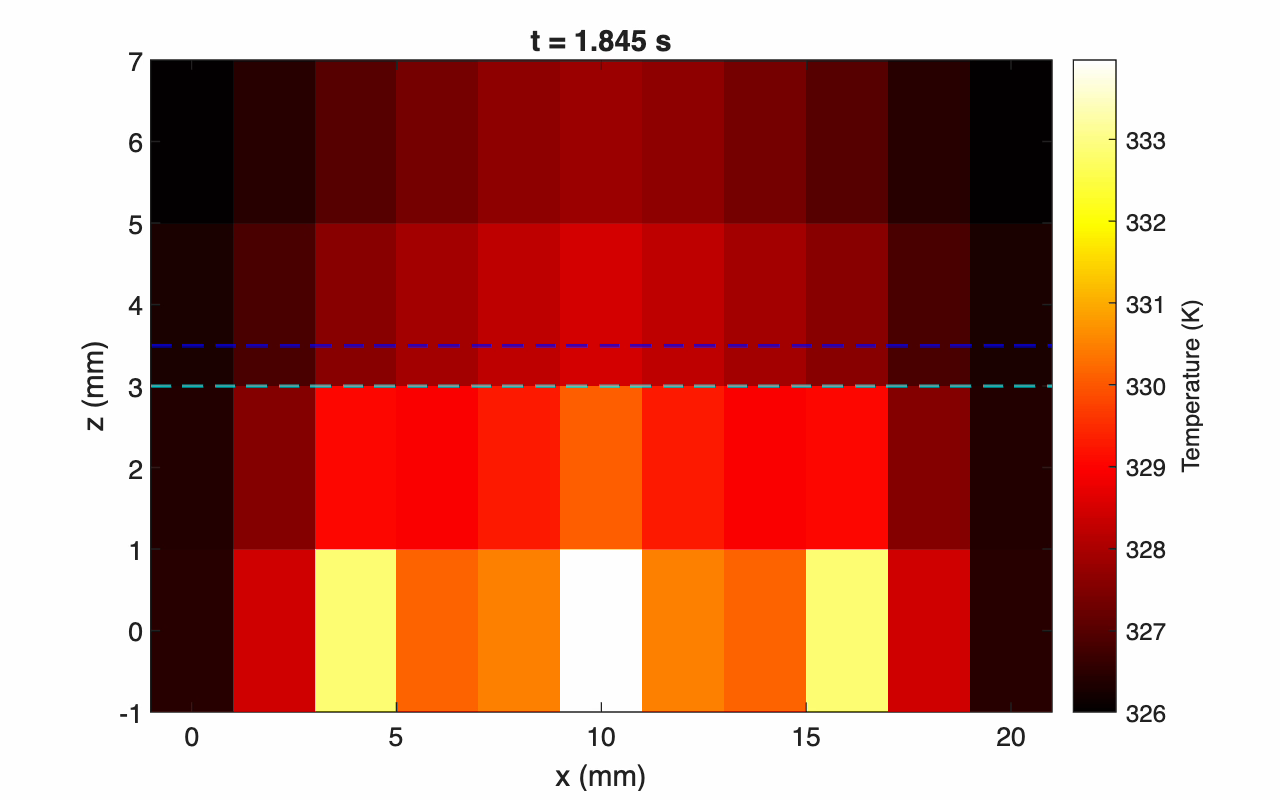
\includegraphics[width=\columnwidth]{fig1_transient_early.png}
  \caption{Explicit FTCS temperature field during early transient heating.
    Three localized hot-spots are visible at the CPU core locations
    ($x = 4$, $10$, $16\,\text{mm}$) within the silicon die.
    Dashed lines mark the Si/TIM (cyan) and TIM/Cu (blue) interfaces.}
  \label{fig:transient}
\end{figure}

\subsection{Steady-State Temperature Distribution}

All three solvers converge to the same steady-state field, providing
mutual validation. The peak steady-state junction temperature at the
CPU cores reaches approximately $380$--$420\,\text{K}$, depending on
lateral position. The center core runs slightly hotter than the outer
cores due to reduced lateral conduction pathways.

The copper spreader maintains a nearly uniform temperature at its top
surface, demonstrating its effectiveness as a thermal diffusion layer.
The maximum temperature gradient across the TIM is approximately
$15$--$25\,\text{K/mm}$, consistent with the material's relatively
low $k$ value.

Figure~\ref{fig:steady} shows the near-steady-state temperature field
from the explicit solver. The lateral spreading effect of the copper
layer is evident in the more uniform colour distribution near the top
of the domain.

\begin{figure}[H]
  \centering
  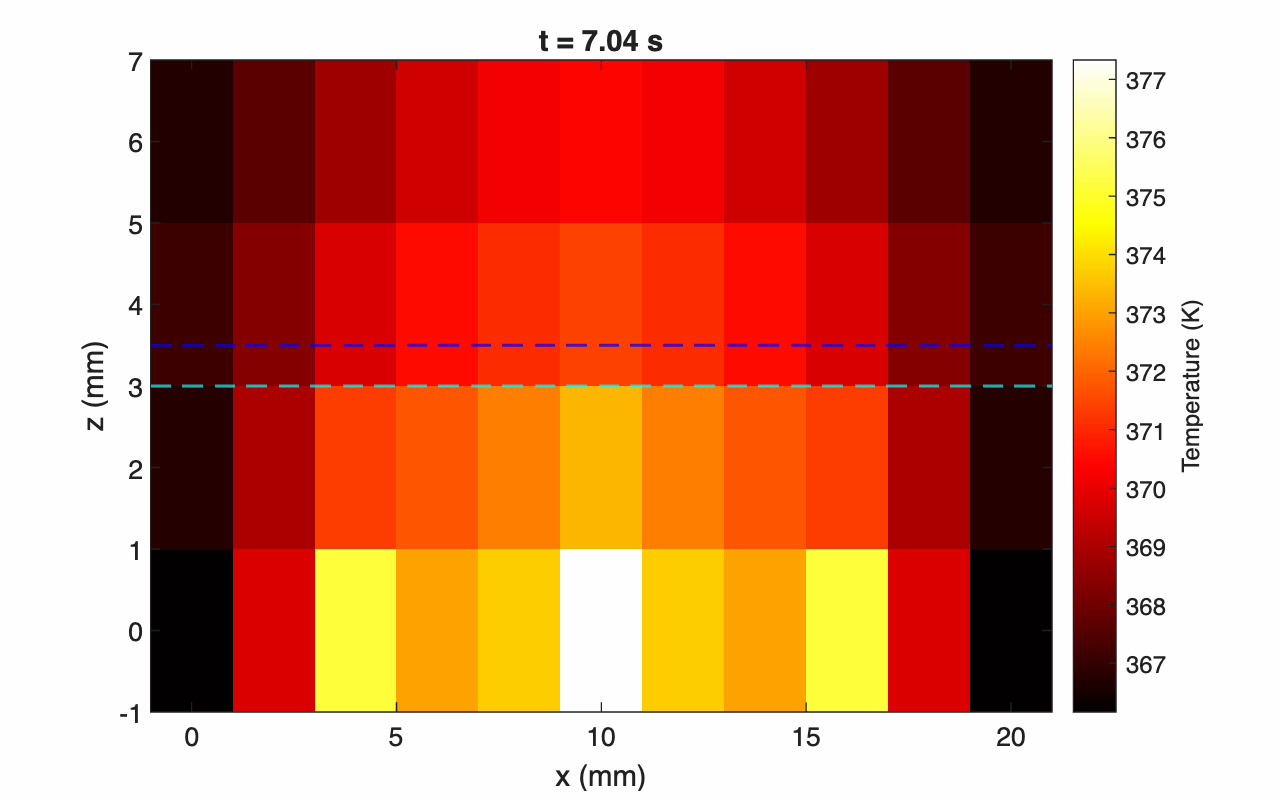
\includegraphics[width=\columnwidth]{fig2_steady_state.png}
  \caption{Temperature field near steady state (explicit FTCS).
    The copper heat spreader distributes heat laterally, producing a
    more uniform top-surface temperature compared to the concentrated
    hot-spots in the silicon die.}
  \label{fig:steady}
\end{figure}

Figure~\ref{fig:comparison} presents a three-panel comparison of the
explicit, steady-state, and implicit solutions at the same time instant,
confirming solver agreement.

\begin{figure}[H]
  \centering
  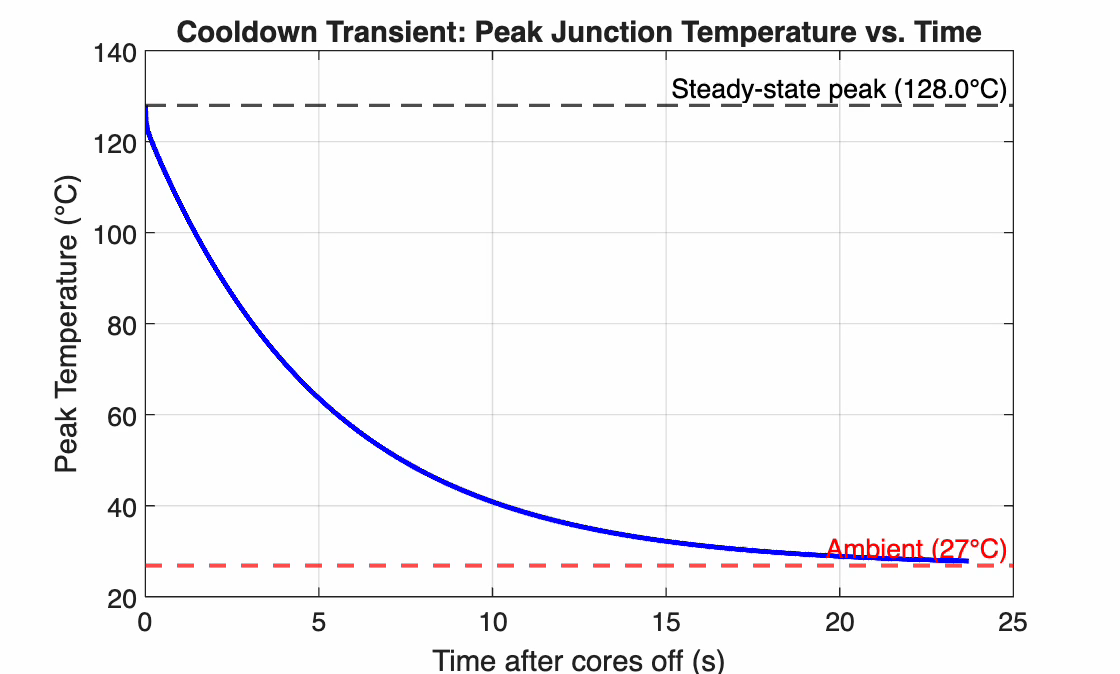
\includegraphics[width=\columnwidth]{fig3_solver_comparison.png}
  \caption{Three-panel solver comparison: explicit FTCS (left),
    steady-state Gauss--Seidel (centre), and implicit BTCS (right).
    All three methods produce consistent temperature distributions,
    validating the numerical implementation.}
  \label{fig:comparison}
\end{figure}

\subsection{Cool-Down Phase}

After the heat sources are deactivated, the chip returns to ambient
temperature. The copper spreader cools more slowly than the silicon die:
despite its higher diffusivity, its greater thermal mass ($\rho c_p V$)
stores more energy. The peak-temperature cool-down follows an
approximately exponential decay toward $T_\infty$.

\begin{figure}[H]
  \centering
  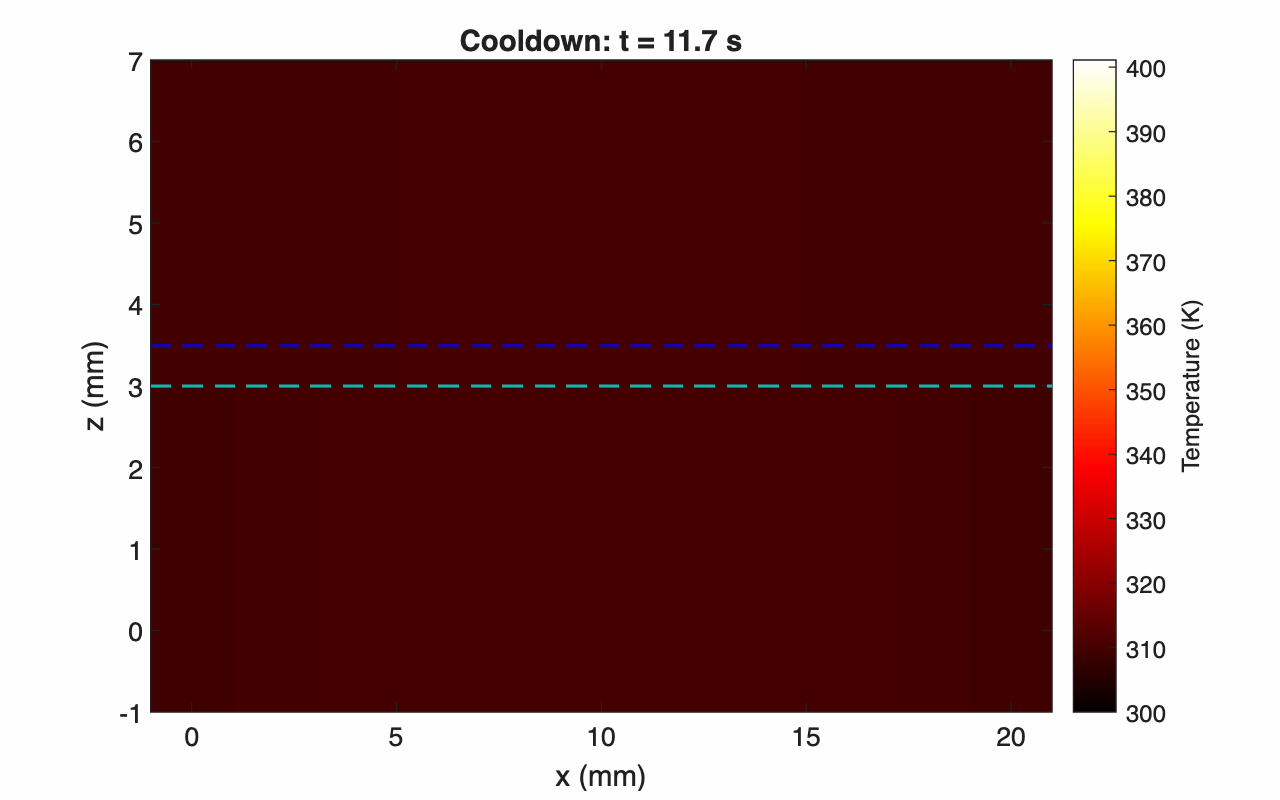
\includegraphics[width=\columnwidth]{fig4_cooldown.png}
  \caption{Temperature field during the cool-down phase after heat
    sources are switched off. The chip stack relaxes toward ambient
    ($\SI{300}{K}$), with the copper spreader retaining heat longer
    due to its higher thermal mass.}
  \label{fig:cooldown}
\end{figure}

\subsection{Solver Comparison}

Table~\ref{tab:solvers} summarizes the key trade-offs among the three
methods.

\begin{table}[H]
  \centering
  \caption{Comparison of numerical solvers.}
  \label{tab:solvers}
  \small
  \begin{tabularx}{\columnwidth}{@{}lXX@{}}
    \toprule
    Solver & Strengths & Limitations \\
    \midrule
    Explicit FTCS
      & Simple implementation; straightforward for animations
      & Small $\Delta t$ required; many steps \\[3pt]
    Implicit BTCS
      & Unconditionally stable; large $\Delta t$ allowed
      & Iterative solve per step; more complex \\[3pt]
    Steady-State GS
      & Fast final-state solution; no time marching
      & No transient information \\
    \bottomrule
  \end{tabularx}
\end{table}

The explicit and implicit transient results agree to within
$\Delta T < \SI{0.5}{K}$ at corresponding time instants, and both
converge to the steady-state solution, confirming correctness.

% ==============================================================================
\section{Conclusion}
% ==============================================================================

A 2D finite difference thermal simulation of a CPU/GPU chip package was
implemented in MATLAB using three solvers: explicit FTCS, implicit BTCS,
and steady-state Gauss--Seidel. Key findings:

\begin{enumerate}[leftmargin=*,label=\arabic*.]
  \item The copper heat spreader is essential for reducing hot-spot
    temperatures. Without lateral spreading, the silicon die would
    sustain higher peak temperatures concentrated directly above each core.
  \item The TIM layer is the dominant thermal resistance in the stack.
    Even a modest improvement in TIM conductivity (e.g., from
    \SI{5}{W/m.K} to \SI{10}{W/m.K}) would substantially reduce
    junction temperature.
  \item Peak junction temperatures under the modeled heat flux remain near
    $\SI{420}{K}$, within typical safe operating limits for silicon devices
    ($T_{j,\max} \approx \SI{398}{K}$--$\SI{423}{K}$).
  \item All three solvers produce consistent results, validating the
    numerical implementation.
\end{enumerate}

Future extensions include: (i)~temperature-dependent material properties,
(ii)~3D extension to capture package-level spreading, (iii)~varying TIM
thickness as a design parameter, and (iv)~coupling to a fluid convection
model for the forced-air cooling channel.

% ── References ────────────────────────────────────────────────────────────────
\begin{thebibliography}{9}

\bibitem{incropera2011}
T.~L.~Bergman, A.~S.~Lavine, F.~P.~Incropera, and D.~P.~DeWitt,
\textit{Fundamentals of Heat and Mass Transfer}, 7th~ed.
John Wiley \& Sons, Hoboken, NJ, 2011.

\bibitem{cengel2010}
Y.~A.~\c{C}engel and A.~J.~Ghajar,
\textit{Heat and Mass Transfer: Fundamentals and Applications}, 4th~ed.
McGraw-Hill, New York, 2010.

\bibitem{matlab2023}
The MathWorks, Inc.,
\textit{MATLAB R2023b}.
Natick, Massachusetts, 2023.

\bibitem{patankar1980}
S.~V.~Patankar,
\textit{Numerical Heat Transfer and Fluid Flow}.
Hemisphere Publishing, Washington D.C., 1980.

\end{thebibliography}

\end{document}